\documentclass{article}
\usepackage{graphicx} % Required for inserting images
\usepackage{amsmath}
\title{Homework 3 solutions}
\author{Intro to Robotics}
\date{}

\begin{document}

\maketitle

\section{Quaternions}
\textbf{1.} rotate the 3d vector $P_{1}=\begin{bmatrix}
-1  \\
2 \\
3
\end{bmatrix}$ by $175^{\circ}$ on xz plane and then $35^{\circ}$ on the yz plane using quaternions. \\\\
\textbf{Solution: } Using -$>$ $\begin{bmatrix}
a & -b & -c & -d\\
b & a & -d & c\\
c & d & a & -b \\
d & -c & b & a
\end{bmatrix}$ for multiplication we get: \\ 
$q_{rot}=e^{\frac{35^\circ}{2}n_x} e^{\frac{175^\circ}{2}n_y} = \begin{bmatrix}
c \frac{35^\circ}{2} & -s \frac{35^\circ}{2} & 0 & 0\\
s \frac{35^\circ}{2} & c \frac{35^\circ}{2} & 0 & 0\\
0 & 0 & c \frac{35^\circ}{2} & -s \frac{35^\circ}{2} \\
0 & 0 & s \frac{35^\circ}{2} & c \frac{35^\circ}{2}
\end{bmatrix}\begin{bmatrix}
c\frac{175}{2}\\
0\\
s\frac{175}{2}\\
0
\end{bmatrix}=\begin{bmatrix}
.04 \\
.01 \\
0.95 \\
0.3
\end{bmatrix}$\\\\
$P_{1r}=q_{rot}P_1 q_{rot}^*=\begin{bmatrix}
.04 & -.01 & -.95 & -.3\\
.01 & .04 & -.3 & .95\\
.95 & .3 & .04 & -.01\\
.3 & -.95 &  .01 & .04 
\end{bmatrix}\begin{bmatrix}
0\\
-1\\
2\\
3
\end{bmatrix}=\begin{bmatrix}
-2.79\\
2.22\\
-.26\\
1.1
\end{bmatrix}\\\\
\begin{bmatrix}
-2.79 & -2.22 & .26 & -1.1\\
2.22 & -2.79 & -1.1 & -.26\\
-.26 & 1.1 &  -2.79 & -2.22\\
1.1 & .26 &  2.22 & -2.79 
\end{bmatrix}\begin{bmatrix}
.04 \\
-.01 \\
-0.95 \\
-0.3
\end{bmatrix}=\begin{bmatrix}
0\\
1.26\\
3.3\\
-1.23
\end{bmatrix}$\\\\
\textbf{2.} Convert ${}^{A}_{B}R_{Z'Y'X'}(50^\circ, 150^\circ, 200^\circ)$ to quaternion coordinates.\\\\
\textbf{Solution: } $e^{\frac{50^\circ}{2}n_z} e^{\frac{150^\circ}{2}n_y} e^{\frac{200^\circ}{2}n_x} =\\
\begin{bmatrix}
c \frac{50^\circ}{2} & 0 & 0 & -s \frac{50^\circ}{2}\\
0 & c \frac{50^\circ}{2} & s \frac{50^\circ}{2} & 0\\
0 & s \frac{50^\circ}{2} & c \frac{50^\circ}{2} & 0 \\
s \frac{50^\circ}{2} & 0 & 0 & c \frac{50^\circ}{2}
\end{bmatrix}
\begin{bmatrix}
c \frac{150^\circ}{2} & 0 & -s \frac{150^\circ}{2} & 0\\
0 & c \frac{150^\circ}{2} & -s \frac{150^\circ}{2} & 0\\
s \frac{150^\circ}{2} & 0 & c \frac{150^\circ}{2} & 0 \\
0 & s \frac{150^\circ}{2} & 0 & c \frac{150^\circ}{2}
\end{bmatrix}
\begin{bmatrix}
c \frac{200^\circ}{2} & -s \frac{200^\circ}{2} & 0 & 0\\
s \frac{200^\circ}{2} & c \frac{200^\circ}{2} & 0 & 0\\
0 & 0 & c \frac{200^\circ}{2} & -s \frac{200^\circ}{2} \\
0 & 0 & s \frac{200^\circ}{2} & c \frac{200^\circ}{2}
\end{bmatrix}=\begin{bmatrix}
.36\\
.3\\
-.04\\
-.88
\end{bmatrix}$\\\\
\textbf{3.} Convert rotation matrix $R=\begin{bmatrix}
.28 & .77 & .57\\
-.94 & .34 & 0 \\
-.19 & -.54 & .82
\end{bmatrix}$ to quaternion coordinates.\\\\
\textbf{Solution: } First convert Rotation matrix to z'y'x' euler angles:\\
$\beta_2=180^{\circ}-\beta_1=180^{\circ}--arcsin(-.19)=180^{\circ}-10.95=169.05^{\circ}$\\
$\alpha_1=arctan(\frac{r_{21}}{r_{11}})=arctan(\frac{-.18}{-.18})=45^{\circ}$\\
$\alpha_2=arctan(\frac{r_{21}}{r_{11}})=arctan(\frac{-.94}{.28})=-73.41^{\circ}=-73.41+180=106.59^\circ, \frac{r_{11}}{cos(\beta_2)}=\frac{.28}{-.98} < 0$(add 180)\\
$\gamma_2=arctan(\frac{r_{32}}{r_{33}})=arctan(\frac{-.54}{.82})=45^{\circ}=-33.37+180=146.63^\circ, \frac{r_{33}}{cos(\beta_2)}=\frac{.82}{-.98} < 0$(add 180)\\\\
You will always have two sets of possible answers.\\
Set 2: $(\alpha_1, \beta_1, \gamma_1)=(106.59^{\circ}, 169.05^{\circ},146.63 ^{\circ})$\\\\
$e^{\frac{106.59^\circ}{2}n_z} e^{\frac{150^\circ}{2}n_y} e^{\frac{200^\circ}{2}n_x} =\\
\begin{bmatrix}
c \frac{106.59^\circ}{2} & 0 & 0 & -s \frac{106.59^\circ}{2}\\
0 & c \frac{106.59^\circ}{2} & s \frac{106.59^\circ}{2} & 0\\
0 & s \frac{106.59^\circ}{2} & c \frac{50^\circ}{2} & 0 \\
s \frac{106.59^\circ}{2} & 0 & 0 & c \frac{50^\circ}{2}
\end{bmatrix}
\begin{bmatrix}
c \frac{169.05^\circ}{2} & 0 & -s \frac{169.05^\circ}{2} & 0\\
0 & c \frac{169.05^\circ}{2} & -s \frac{169.05^\circ}{2} & 0\\
s \frac{169.05^\circ}{2} & 0 & c \frac{169.05^\circ}{2} & 0 \\
0 & s \frac{169.05^\circ}{2} & 0 & c \frac{169.05^\circ}{2}
\end{bmatrix}\\
\begin{bmatrix}
c \frac{146.63^\circ}{2} & -s \frac{146.63^\circ}{2} & 0 & 0\\
s \frac{146.63^\circ}{2} & c \frac{146.63^\circ}{2} & 0 & 0\\
0 & 0 & c \frac{146.63^\circ}{2} & -s \frac{146.63^\circ}{2} \\
0 & 0 & s \frac{146.63^\circ}{2} & c \frac{146.63^\circ}{2}
\end{bmatrix}=\begin{bmatrix}
.78\\
-.17\\
.24\\
-.55
\end{bmatrix}$\\\\
\textbf{4.} consider quaternion $q_{1}$ = (0.845 +0.191i +0.462j +0.191k), convert to $R_{Z'Y'X'}(\alpha,\beta,\gamma)$.\\\\
\textbf{Solution: }\\ $alpha = arctan2(2*(0.845*0.191+0.462*0.191),1-(2*(0.191^2+0.462^2)) )\\
beta = arcsin(2*(0.845*0.462-0.191^2))\\
gamma = arctan2(2*(0.845*0.191+0.191*0.462),1-(2*(0.462^2+0.191^2)) )$\\\\
\textbf{5.}  Write a function that rotates 3d vectors using quaternions to verify your answers for 1-3.\\\\
\textbf{View Attached in hw3.py and eulerangles.py on blackboard. } \\\\
\textbf{6.} Write a function that takes a rotation matrix as input and returns the equivalent quaternions.\\\\
\textbf{View Attached in hw3.py and eulerangles.py on blackboard. } \\\\
\textbf{7.} Write a function that takes a quaternions as input and returns the equivalent rotation matrix.\\
\textbf{View Attached in hw3.py and eulerangles.py on blackboard. } 
\newpage
\section{Kinematics 1}
\begin{figure}[htp]
    \centering
    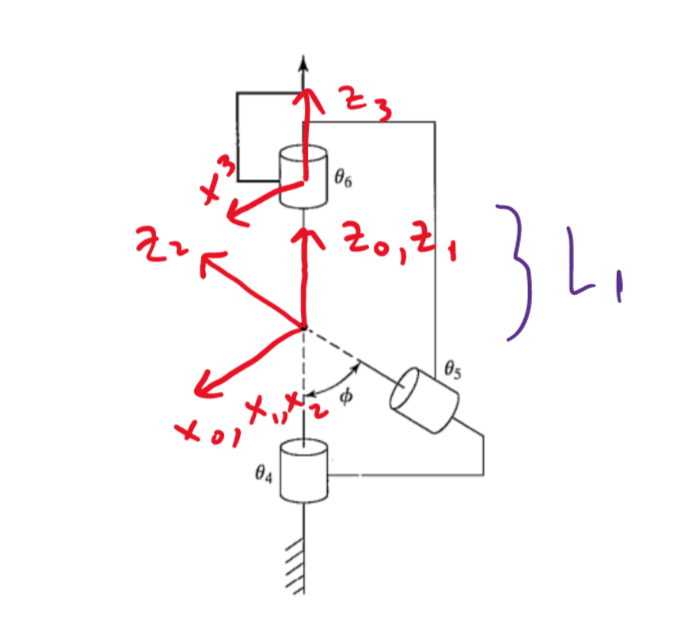
\includegraphics[width=8cm]{kinematics 1 answer.png}
    \caption{}
    \label{fig:Arm}
\end{figure}
\textbf{1.} Compute the frames, dh table and rotation matrices for the given schematic.\\\\
$a_0=dist(z_0,z_1) \text{ in } x_0=0\\
a_1=dist(z_1,z_2) \text{ in } x_1=0\\
a_2=dist(z_2,z_3) \text{ in } x_2=0\\\\
\alpha_0=angle(z_0,z_1) \text{ in } x_0=0\\
\alpha_1=angle(z_1,z_2) \text{ in } x_1=\phi\\
\alpha_2=angle(z_2,z_3) \text{ in } x_2=-\phi\\\\
d_1=dist(x_0,x_1) \text{ in } z_1=0\\
d_2=dist(x_1,x_2) \text{ in } z_2=0\\
d_3=dist(x_2,x_3) \text{ in } z_3=L_1\\\\
\theta_1=angle(x_0,x_1) \text{ in } z_1=\theta_4\\
\theta_2=angle(x_1,x_2) \text{ in } z_2=\theta_5\\
\theta_3=angle(x_2,x_3) \text{ in } z_3=\theta_6$\\\\
\begin{tabular}{ |p{3cm}|p{3cm}|p{3cm}| p{3cm} | p{3cm} |}
\hline
\multicolumn{5}{|c|}{DH table} \\
\hline
Frame \{i\} & \textbf{$a_{i-1}$} & \textbf{$\alpha_{i-1}$} & \textbf{$d_i$} & \textbf{$\theta_i$} \\
\hline
\textbf{1} & 0     & 0 & 0 & $\theta_4$\\
\textbf{2} & 0 & $\phi$ & 0 & $\theta_5$\\
\textbf{3} & 0 & $-\phi$ & $L_1$ & $\theta_6$\\
\hline
\end{tabular}\\\\
Using
${}^{i-1}_{i}T=\begin{bmatrix}
c\theta_i & -s\theta_i & 0 & a_{i-1}\\
s\theta_ic\alpha_{i-1} & c\theta_ic\alpha_{i-1} & -s\alpha_{i-1} & -s\alpha_{i-1}d_{i}\\
s\theta_is\alpha_{i-1} & c\theta_is\alpha_{i-1} & c\alpha_{i-1} & c\alpha_{i-1}d_{i}\\
                0 & 0 & 0 & 1
\end{bmatrix}$ we get. Tip-Each row corresponds to one transformation matrix:\\\\
${}^{0}_{1}T=
\begin{bmatrix}
c\theta_4 & -s\theta_4 & 0 & 0\\
s\theta_4 & c\theta_4 & 0 & 0\\
0 & 0 & 1 & 0\\
0 & 0 & 0 & 1
\end{bmatrix}$\\\\
${}^{1}_{2}T=
\begin{bmatrix}
c\theta_5 & -s\theta_5 & 0 & 0\\
s\theta_5c\phi & c\theta_5c\phi & -s\phi & 0\\
s\theta_5s\phi & c\theta_5s\phi & c\phi & 0\\
0 & 0 & 0 & 1
\end{bmatrix}$\\\\
${}^{2}_{3}T=
\begin{bmatrix}
c\theta_6 & -s\theta_6 & 0 & 0\\
s\theta_6c-\phi & c\theta_6c-\phi & -s-\phi & -s-\phi L_1\\
s\theta s-\phi & c\theta s-\phi & c-\phi & c-\phi L_1\\
0 & 0 & 0 & 1
\end{bmatrix}$
\newpage

\section{Kinematics 2}
\begin{figure}[htp]
    \centering
    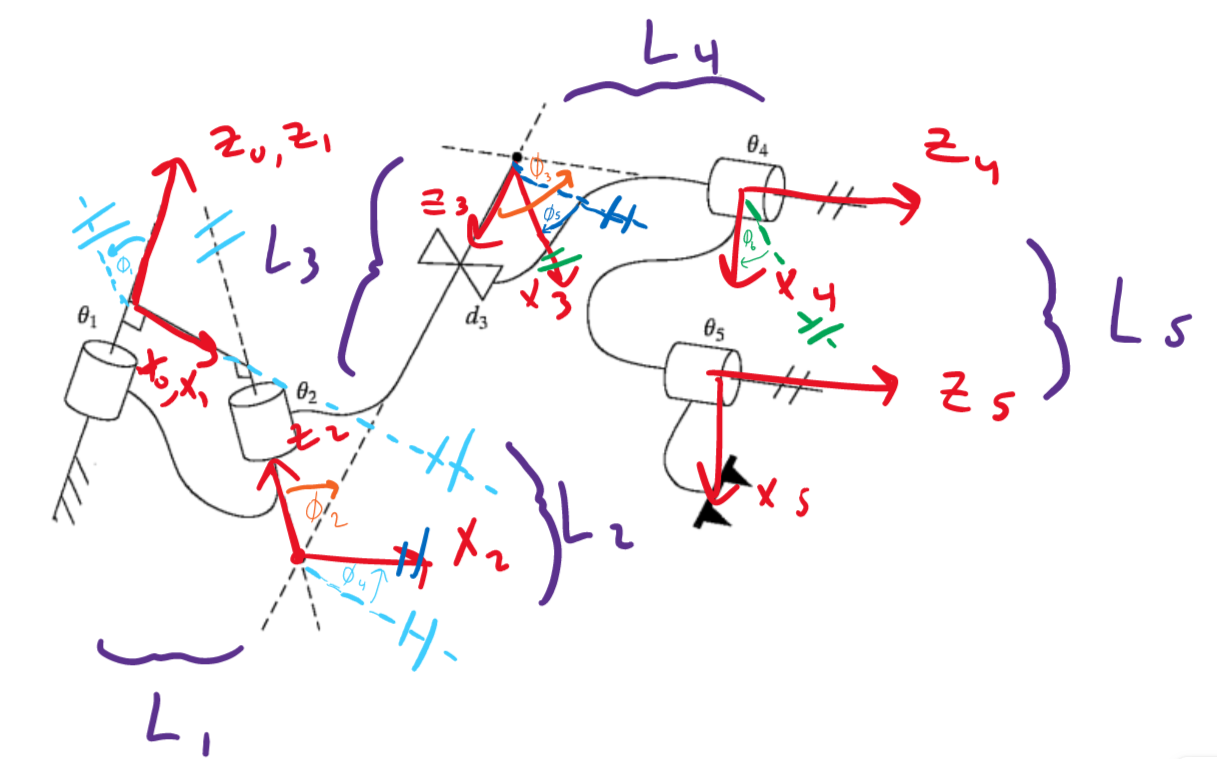
\includegraphics[width=12cm]{kinematics 2 answer.png}
    \caption{}
    \label{fig:Arm}
\end{figure}
\textbf{1.} Compute the frames, dh table and rotation matrices for the given schematic.\\\\
$a_0=dist(z_0,z_1) \text{ in } x_0=0\\
a_1=dist(z_1,z_2) \text{ in } x_1=L_1\\
a_2=dist(z_2,z_3) \text{ in } x_2=0\\
a_3=dist(z_3,z_4) \text{ in } x_3=0\\
a_4=dist(z_4,z_5) \text{ in } x_4=L_5\\\\
\alpha_0=angle(z_0,z_1) \text{ in } x_0=0\\
\alpha_1=angle(z_1,z_2) \text{ in } x_1=\phi_1\\
\alpha_2=angle(z_2,z_3) \text{ in } x_2=\phi_2\\
\alpha_3=angle(z_3,z_4) \text{ in } x_3=\phi_3\\
\alpha_4=angle(z_4,z_5) \text{ in } x_4=0\\\\
d_1=dist(x_0,x_1) \text{ in } z_1=0\\
d_2=dist(x_1,x_2) \text{ in } z_2=L_2\\
d_3=dist(x_2,x_3) \text{ in } z_3=L_3-d_3\\
d_4=dist(x_3,x_4) \text{ in } z_4=L_4\\
d_5=dist(x_4,x_5) \text{ in } z_5=0\\\\
\theta_1=angle(x_0,x_1) \text{ in } z_1=\theta_1\\
\theta_2=angle(x_1,x_2) \text{ in } z_2=\theta_2-\phi_4\\
\theta_3=angle(x_2,x_3) \text{ in } z_3=\phi_5\\
\theta_4=angle(x_3,x_4) \text{ in } z_4=\theta_4-\phi_6\\
\theta_5=angle(x_4,x_5) \text{ in } z_5=\theta_5$\\\\
\begin{tabular}{ |p{3cm}|p{3cm}|p{3cm}| p{3cm} | p{3cm} |}
\hline
\multicolumn{5}{|c|}{DH table} \\
\hline
Frame \{i\} & \textbf{$a_{i-1}$} & \textbf{$\alpha_{i-1}$} & \textbf{$d_i$} & \textbf{$\theta_i$} \\
\hline
\textbf{1} & 0     & 0 & 0 & $\theta_1$\\
\textbf{2} & $L_1$ & $\phi_1$ & $L_2$ & $\theta_2-\phi_4$\\
\textbf{3} & 0 & $\phi_2$ & $L_3-d_3$ & $\phi_5$\\
\textbf{4} & 0 & $\phi_3$ & $L_4$ & $\theta_4-\phi_6$\\
\textbf{5} & $L_5$ & 0 & 0 & $\theta_5$\\
\hline
\end{tabular}\\\\
Using
${}^{i-1}_{i}T=\begin{bmatrix}
c\theta_i & -s\theta_i & 0 & a_{i-1}\\
s\theta_ic\alpha_{i-1} & c\theta_ic\alpha_{i-1} & -s\alpha_{i-1} & -s\alpha_{i-1}d_{i}\\
s\theta_is\alpha_{i-1} & c\theta_is\alpha_{i-1} & c\alpha_{i-1} & c\alpha_{i-1}d_{i}\\
                0 & 0 & 0 & 1
\end{bmatrix}$ we get:\\\\
${}^{0}_{1}T=
\begin{bmatrix}
c\theta_1 & -s\theta_1 & 0 & 0\\
s\theta_1 & c\theta_1 & 0 & 0\\
0 & 0 & 1 & 0\\
0 & 0 & 0 & 1
\end{bmatrix}$\\\\
${}^{1}_{2}T=
\begin{bmatrix}
c(\theta_2-\phi_4) & -s(\theta_2-\phi_4) & 0 & L_1\\
s(\theta_2-\phi_4)c\phi_1 & c(\theta_2-\phi_4)c\phi_1 & -s\phi_1 & -s\phi_1L_2\\
s(\theta_2-\phi_4)s\phi_1 & c(\theta_2-\phi_4)s\phi_1 & c\phi_1 & c\phi_1L_2\\
0 & 0 & 0 & 1
\end{bmatrix}$\\\\
${}^{2}_{3}T=
\begin{bmatrix}
c\phi_5 & -s\phi_5 & 0 & 0\\
s\phi_5c\phi_2 & c\phi_5c\phi_2 & -s\phi_2 & -s\phi_2*(L_3-d_3)\\
s\phi_5s\phi_2 & c\phi_5s\phi_2 & c\phi_2 & c\phi_2*(L_3-d_3)\\
0 & 0 & 0 & 1
\end{bmatrix}$\\\\
${}^{3}_{4}T=
\begin{bmatrix}
c(\theta_4-\phi_6) & -s(\theta_4-\phi_6) & 0 & 0\\
s(\theta_4-\phi_6)c\phi_3 & c(\theta_4-\phi_6)c\phi_3 & -s\phi_3 & -s\phi_3L_4\\
s(\theta_4-\phi_6)s\phi_3 & c(\theta_4-\phi_6)s\phi_3 & c\phi_3 & c\phi_3L_4\\
0 & 0 & 0 & 1
\end{bmatrix}$\\\\
${}^{4}_{5}T=
\begin{bmatrix}
c\theta_5 & -s\theta_5 & 0 & L_5\\
s\theta_5 & c\theta_5 & 0 & 0\\
0 & 0 & 1 & 0\\
0 & 0 & 0 & 1
\end{bmatrix}$
\end{document}
